
\documentclass{beamer}

\usepackage[utf8]{inputenc}
\usepackage[spanish]{babel}
\usepackage{animate}

\usepackage{beamerthemesplit}

\usetheme{Warsaw} 

\title{Redes neuronales multicapa}
\subtitle{Castiglione, Karpovsky, Sturla }
\author{Sistemas de Inteligencia Artificial}
\date{3 de Mayo de 2012}

\AtBeginSection[]
{
  \begin{frame}{Tabla de contenidos}
    \tableofcontents[currentsection]
  \end{frame}
}


\begin{document}

\frame{\titlepage}

\section[Outline]{}
\frame{\tableofcontents}

\section{Introducción}
\subsection{El problema}
\begin{frame}{El problema}


\par El problema consistió en analizar el comportamiento de una Red de hopfield como memoria asociativa direccionable por el contenido.\\
\begin{itemize}
\item Red de Hopfield implementada en el lenguaje \textit{Java}.
\end{itemize}
\end{frame}

\begin{frame}{Modelado del problema}

\par Algunas definiciones preliminares:\\
\begin{itemize}
\item \textbf{$\Psi$}: Conjunto de patrones a memorizar
\item \textbf{$N$}: Longitud de los patrones de entrada (ej. $N = 64$ si cada imagen es de $8x8$ pixels)
\item \textbf{$p$}: Cantidad de patrones distintos que contiene $\Psi$\\
\end{itemize}

\par Se representó a la Red de Hopfield  como una clase abstracta debido a la distinción entre el algoritmo \textbf{sincrónico} y el algoritmo \textbf{asincrónico}.\\
\end{frame}

\begin{frame}{Patrones}

\begin{figure}[H]
\begin{center}
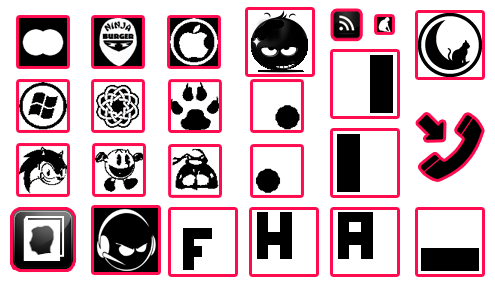
\includegraphics[scale=0.40]{./images/patterns.png}
\label{modelado}
\end{center}
\end{figure}

\begin{center}
\par Figura 1: Visualización de los 25 patrones con la que se inicializa a la red
\end{center}

\end{frame}

\begin{frame}{Modelado del problema}

La clase contiene dos variables: un vector y una matriz que están definidos como sigue:\\

\begin{itemize}
\item \textbf{float[N][N] weights}: Matriz de pesos $w_{ij}$ correspondientes a los patrones que se desean memorizar.
\item \textbf{int[N] states}: Vector con los estados de cada una de las $N$ neuronas.\\
\end{itemize}

\par Nótese que si bien el vector de estados es de tipo entero, los estados definidos para este problema son $1$ o $-1$ dado que las unidades que están siendo utilizadas son \textbf{bipolares}.\\

\end{frame}

\begin{frame}{Modelado del problema}
\begin{itemize}
\item Representación de $\mu$\\
\end{itemize}

\par Representar a los patrones $\mu$ como vectores de enteros \textbf{\textit{int[] pattern}} los cuales contienen un $1$ en la posición $i$ en el caso de que el i-ésimo pixel del patrón sea negro o contienen un $-1$ en la posición $i$ en el caso de que el i-ésimo pixel del patrón sea blanco.\\

\begin{itemize}
\item Los patrones fueron \textit{normalizados} (escala de grises a B\&W)
\end{itemize}

\end{frame}


\section{Redes Neuronales}

\subsection{Inicialización de la red}

\begin{frame}{Inicialización de la red}

\par El método \textit{storePatterns} inicializa la matriz de pesos sinápticos de la red utilizando la regla del producto externo de \textbf{Hebb}.\\
\par Nótese que la matriz de pesos, una vez inicializada, no cambia durante toda la ejecución del algoritmo.\\

\begin{itemize}
\item \textbf{Simetría:} La matriz de pesos es simétrica con $w_{ij} = 0$
\item \textbf{Matriz de pesos:} Una vez inicializada queda estática.
\end{itemize}
\end{frame}

\begin{frame}{Función de activación}

\par La función de activación utizada es la función signo: \textbf{f(x) = x}.

\end{frame}

\begin{frame}{Actualización de estados}

\begin{block}{Regla de actualización}

\[
S_i(n+1) = sgn\left(\sum_{j=1}^{N}{W_{ij}S_j(n)}\right)
\]

\end{block}
\vspace{10px}
\par La convergencia está dada cuando el vector de estados permanece invariante respecto del vector en el paso anterior o se detecte un \textbf{ciclo de longitud dos} en las actualizaciones del vector de estados.\\

\end{frame}

\subsection{Red sincrónica: Modelo de Little}
\begin{frame}{Red sincrónica: Modelo de Little}

\par Se implementó una red neuronal con el modelo de \textbf{Little} en la cual la actualización de los estados es sincrónica.

\end{frame}

\begin{frame}{Actualización de estados}

\begin{itemize}
\item Actualizar todas las neuronas simultaneamente en cada paso.
\end{itemize}

\end{frame}

\subsection{Red asincrónica: Modelo de Hopfield}
\begin{frame}{Red asincrónica: Modelo de Hopfield}

\par Se implementó una red neuronal con el modelo de \textbf{Hopfield} en la cual la actualización de los estados es asincrónica.

\end{frame}

\begin{frame}{Actualización de estados}

\begin{itemize}
\item En cada paso se actualiza de a una unidad por vez, la misma es elegida al azar.
\end{itemize}

\end{frame}


\subsection{Mejoras implementadas}

\begin{frame}{Mejoras implementadas}

\begin{itemize}
\item \Large Bit de paridad
\item \Large Matriz pseudo-inversa

\end{itemize}
\end{frame}

\begin{frame}{Matriz pseudo-inversa}

\par El cálculo de la matriz pseudo-inversa viene dado por:

\begin{block}{Cálculo de matriz pseudo-inversa}

\[
w_{ij}=\frac{1}{N}\sum_{\mu \nu} \xi_i^{\mu}(Q^{-1})_{\mu \nu}  \xi_j^{\nu}
\]

siendo

\[
Q_{\mu \nu} = \frac{1}{N}\sum_{i}  \xi_i^{\mu}  \xi_i^{\nu}
\]

\end{block}
\end{frame}

\begin{frame}{Matriz pseudo-inversa}

\par El error de la imagen que se obtiene como respuesta está dado por: \\
\vspace{20px}
\begin{block}{Cálculo del error}


\[
error = \frac{bits\_incorrectos}{bits\_totales}
\]


\end{block}
\end{frame}


\section{Resultados}

\subsection{Estados espúreos}
\begin{frame}{Estados espúreos}

\par Se utilizó una red asincrónica y se la hizo memorizar 14 imágenes distintas. 
El resultado de pasarle como entrada la imagen ``line1'' se puede observar a continuación:\\

\begin{figure}[H]
\begin{center}
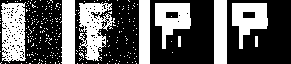
\includegraphics[scale=0.60]{./images/espureo.png}
\label{modelado}
\end{center}
\end{figure}

\begin{center}
\par Figura 1: Ejemplo de estado espúreo.
\end{center}

\end{frame}

\subsection{Patrones con ruido o incompletos}
\begin{frame}{Patrones con ruido o incompletos}


\par Se utilizó una red asincrónica y se la hizo memorizar los archivos ``foot'', ``line1'', ``line2'', ``line3'', ``line4''.\\

A continuación se muestra el resultado de pasarle como entrada la imagen ``foot'' pero incompleta.\\

\begin{figure}[H]
\begin{center}

\includegraphics[scale=0.60]{./images/half.png}
\label{modelado}
\end{center}
\end{figure}

\begin{center}
\par Figura 1: Respuesta de una red de hopfield asincrónica ante un patrón incompleto.
\end{center}

\end{frame}

\begin{frame}{Patrones con ruido o incompletos}

\par Si en cambio se utiliza solamente ruido en una red asincrónica que memorizó los patrones ``f'', ``h'', ``a'', ``footprint'' y le pedimos que evolucione partiendo de ``f'', la red rápidamente converge a la imagen deseada:

\begin{figure}[H]
\begin{center}
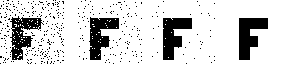
\includegraphics[scale=0.60]{./images/noisyf.png}
\label{modelado}
\end{center}
\end{figure}

\begin{center}
\par Figura 1: Respuesta de una red de hopfield asincrónica ante un patrón con ruido.
\end{center}

\end{frame}

\subsection{Patrones invertidos}

\begin{frame}{Patrones invertidos}

\par Red inicializada con las siguientes imágenes provistas por la cátedra: ``line1'', ``line2'', ``line3'', ``line4'', ``h''.\\

\begin{itemize}
\item Mejora del bit de paridad
\item Mejora de pseudo-inversa
\item Patrón de entrada invertido y con ruido
\end{itemize}

\begin{figure}[H]
\begin{center}

\includegraphics[scale=0.55]{./images/hinvypar.png}
\label{modelado}
\end{center}
\end{figure}

\begin{center}
\par Figura 1: Estados intermedios para una red de hopfield asincrónica con la mejora del bit de paridad y la utilización de la matriz pseudo-inversa
\end{center}
\end{frame}

\subsection{Patrones desconocidos}
\begin{frame}{Patrones desconocidos}

\par El siguiente ejemplo muestra la respuesta de la red ante un patrón desconocido. Se utilizó una red asincrónica y se la hizo memorizar los archivos ``line1'', ``line2'', ``line3'', ``line4''\\.\\
A continuación se muestra el resultado de pasarle como entrada la imagen ``h''  la cual la red no conocía: \\

\begin{figure}[H]
\begin{center}

\includegraphics[scale=0.60]{./images/hnoinvnopar.png}
\label{modelado}
\end{center}
\end{figure}

\begin{center}
\par Figura 2: Respuesta de una red de hopfield asincrónica ante un patrón desconocido.
\end{center}
\end{frame}

\section{Conclusiones}

\begin{frame}{Cantidad de patrones almacenables}

\begin{itemize}
\item \Large La capacidad sugerida por \textit{Hertz} ($0.138N$) no fue verificada, en la práctica fue mucho menor.
\item La red logró almacenar hasta 6 o 7 imágenes.
\end{itemize}

\end{frame}

\end{document}
